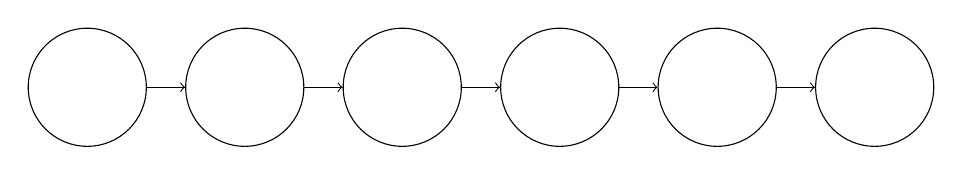
\begin{tikzpicture}[node distance=2cm, every node/.style={draw, circle, minimum size=1.5cm}]
    \node (sunny1) {\Sun};
    \node[right of=sunny1] (sunny2) {\HalfSun};
    \node[right of=sunny2] (partlycloudy) {\SunCloud};
    \node[right of=partlycloudy] (cloudy) {\Cloud};
    \node[right of=cloudy] (rainy) {\RainCloud};
    \node[right of=rainy] (sunny3) {\Sun};
    
    % Arrows
    \draw[->] (sunny1) -- (sunny2);
    \draw[->] (sunny2) -- (partlycloudy);
    \draw[->] (partlycloudy) -- (cloudy);
    \draw[->] (cloudy) -- (rainy);
    \draw[->] (rainy) -- (sunny3);
\end{tikzpicture}